% Homework report template for courses lectured by Blaz Zupan.
% For more on LaTeX please consult its documentation pages, or
% read tutorials like http://tobi.oetiker.ch/lshort/lshort.pdf.
%
% Use pdflatex to produce a PDF of a report.

\documentclass[a4paper,11pt]{article}
\usepackage{a4wide}
\usepackage{fullpage}
\usepackage[toc,page]{appendix}
\usepackage[pdftex]{graphicx} % for figures
\usepackage{setspace}
\usepackage{color}
\definecolor{light-gray}{gray}{0.95}
\usepackage{listings} % for inclusion of Python code
\usepackage{hyperref}
\renewcommand{\baselinestretch}{1.2}

\lstset{ % style for Python code, improve if needed
language=Python,
basicstyle=\footnotesize,
basicstyle=\ttfamily\footnotesize\setstretch{1},
backgroundcolor=\color{light-gray},
}

\title{Evolutionary Tree}
\author{Zidar Miha (63060317)}
\date{\today}

\begin{document}

\maketitle

\section{Introduction}

The goal of this assignment was to download and compare a few mitochondrial sequences, based on \textit{COX3} gene, with \textit{Needleman-Wunsch} algorithm and to construct a dendrogram. The algorithm used a \textit{Blosum50} table and a linear gap penalty.

\section{Data}

We used sequences of 14 different animals, show in the Animal table \ref{animalTable}, that we downloaded from \url{http://www.ncbi.nlm.nih.gov/genbank/}. From the entire mitochondrial genome, we took out only \textit{COX3} gene for comparison. We also used the \textit{BloSum50} table, for getting the comparison costs for all Amino Acid pairs. You can find all \textit{BloSum} tables at \url{ftp://ftp.ncbi.nih.gov/blast/matrices/}


\begin{table}[htbp]
\caption{Table of animal species used.}
\label{animalTable}
\begin{center}
\begin{tabular}{rllp{6cm}}
\hline
Index & GeneBank id & English name & Latin name\\
\hline
  1 &   NC\_000845.1 &                        pig &                     Sus scrofa \\
  2 &   NC\_004299.1 &              Fugu rubripes &              Takifugu rubripes \\ 
  3 &   AC\_000022.2 &                 Norway rat &              Rattus norvegicus \\
  4 &   NC\_002083.1 &         Sumatran orangutan &                   Pongo abelii \\
  5 &   NC\_001643.1 &                 chimpanzee &                Pan troglodytes \\
  6 &   NC\_011137.1 &                 Neandertal &  Homo sapiens neanderthalensis \\
  7 &   NC\_012920.1 &                      human &                   Homo sapiens \\
  8 &   NC\_001645.1 &            western gorilla &                Gorilla gorilla \\
  9 &   NC\_002008.4 &                        dog &         Canis lupus familiaris \\
 10 &   NC\_006580.1 &                   goldfish &      Carassius auratus auratus \\
 11 &   NC\_012420.1 &           veiled chameleon &          Chamaeleo calyptratus \\
 12 &   NC\_011391.1 &            Russell's viper &               Daboia russellii \\
 13 &   NC\_012061.1 &  Longbeaked common dolphin &             Delphinus capensis \\
 14 &   NC\_001640.1 &                      horse &                 Equus caballus 

\\
\hline
\end{tabular}
\end{center}
\end{table}


\section{Methods}

We used \textit{Needleman-Wunsch} algorithm with a fixed linear gap penalty $d=-11$ and \textit{Blosum50} scoring matrix, for global alignment of two sequences.\\

Here we have a simple pseudocode implementation of the \textit{Needleman-Wunsch} algorithm

\begin{lstlisting}
  for i=0 to len(s)
    F(i,0) := d*i
  for j=0 to len(t)
    F(0,j) := d*j
  for i=1 to len(s)
    for j=1 to len(t)
    {
      Match := F(i-1,j-1) + S(s[i], t[j])
      Delete := F(i-1, j) + d
      Insert := F(i, j-1) + d
      F(i,j) := max(Match, Insert, Delete)
    }
\end{lstlisting}
Where $s$ and $t$ are input strings, $S$ is the blosum cost table and $F$ is our cost Matrix. The final comparison score is stored in the last element of $F$ matrix on $F[len(s),len(t)]$.\\

Testing the algorithm with different gap penalties didn't show any significant difference, if we kept the penalty withing the absolute bound of the maximum absolute value in the \textit{Blosum50} matrix. 


\section{Results}

Here we have a pairwise score comparions of all 14 animals (see Table~\ref{scoreTab}) and a dendrogram showing the animals in groups in acordance to their smimilarity score. Provide reference to every table from main text, just like we did in the previous sentence. Notice that Tables should not include vertical lines, and should include horizontal lines only to separate the header from the content and to indicate the end of the table.




\begin{table}[htbp]
\footnotesize
\label{scoreTab}
\begin{center}
\begin{tabular}{r|rrrrrrrrrrrrrr}
1. & 1814 &      &      &      &      &      &      &      &      &      &      &      &      &     \\
2. & 1574 & 1826 &      &      &      &      &      &      &      &      &      &      &      &     \\
3. & 1641 & 1545 & 1816 &      &      &      &      &      &      &      &      &      &      &     \\
4. & 1592 & 1531 & 1586 & 1804 &      &      &      &      &      &      &      &      &      &     \\
5. & 1613 & 1564 & 1643 & 1703 & 1820 &      &      &      &      &      &      &      &      &     \\
6. & 1597 & 1535 & 1614 & 1702 & 1766 & 1816 &      &      &      &      &      &      &      &     \\
7. & 1622 & 1546 & 1625 & 1713 & 1777 & 1798 & 1823 &      &      &      &      &      &      &     \\
8. & 1603 & 1542 & 1611 & 1727 & 1757 & 1753 & 1764 & 1814 &      &      &      &      &      &     \\
9. & 1665 & 1555 & 1672 & 1567 & 1603 & 1585 & 1608 & 1570 & 1832 &      &      &      &      &     \\
10. & 1582 & 1743 & 1552 & 1551 & 1600 & 1574 & 1585 & 1583 & 1556 & 1824 &      &      &      &     \\
11. & 1305 & 1305 & 1320 & 1264 & 1291 & 1278 & 1299 & 1307 & 1296 & 1305 & 1827 &      &      &     \\
12. & 1401 & 1414 & 1405 & 1386 & 1409 & 1395 & 1406 & 1422 & 1381 & 1417 & 1290 & 1796 &      &     \\
13. & 1698 & 1547 & 1628 & 1580 & 1622 & 1615 & 1640 & 1607 & 1682 & 1553 & 1329 & 1395 & 1826 &     \\
14. & 1718 & 1556 & 1658 & 1585 & 1606 & 1604 & 1615 & 1608 & 1688 & 1564 & 1310 & 1410 & 1685 & 1815\\

\hline
 & 1. & 2. & 3. & 4. & 5. & 6. & 7. & 8. & 9. & 10. & 11. & 12. & 13. & 14. \\

\end{tabular}
\caption{Table comparison scores for all animal pairs. See Animal table \ref{animalTable} for index description}
\end{center}
\end{table}


\begin{figure}[htbp]
\begin{center}
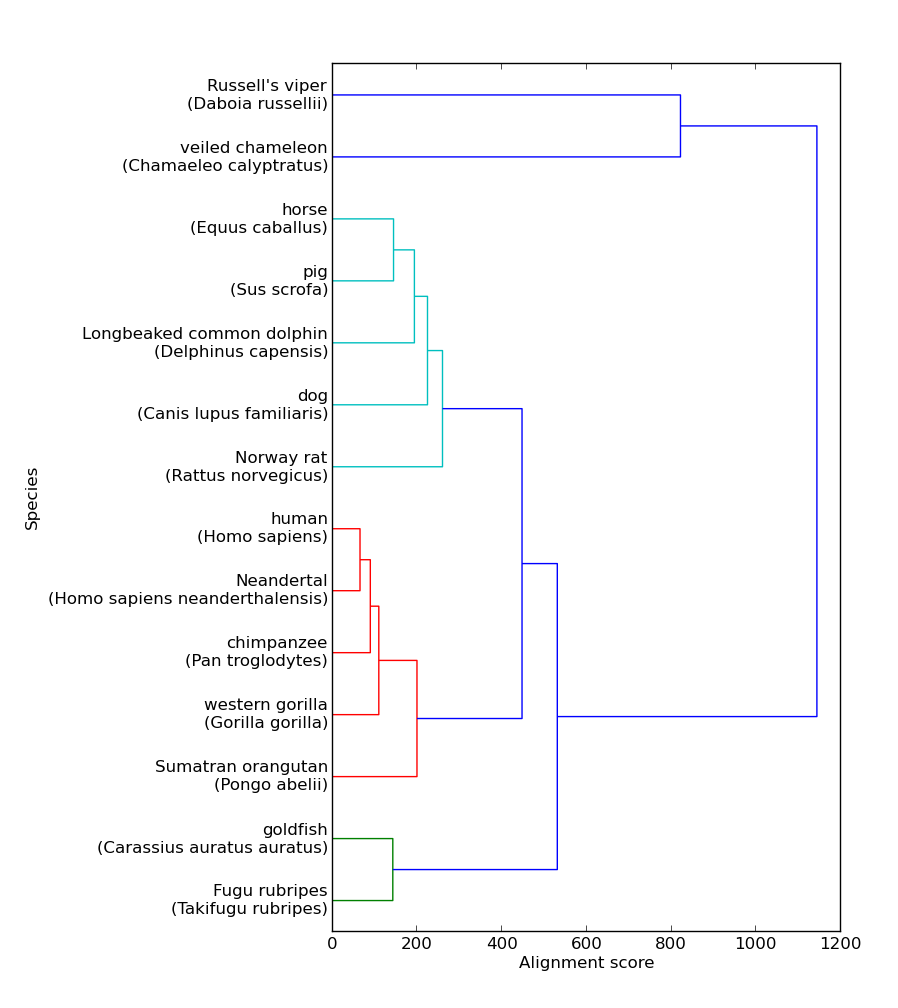
\includegraphics[scale=0.6]{img/dendrogram-gap-11.png}
\caption{Every figure should include a caption with a figure description.}
\label{fig-example}
\end{center}
\end{figure}


\subsection*{Honor Code}

% The following paragraph of your report should be included as is - do % not change it.

My answers to homework are my own work. I did not make solutions or code available to anyone else. I did not engage in any other activities that will dishonestly improve my results or dishonestly improve/hurt the results of others.

\end{document}
